    \subsection{Preliminary Regression}
    Let's regress the following model with OLS:
    \begin{equation}
        V_{t+1} = \beta_0 + \beta_1 V_t
    \end{equation}
    where $V_t=N_t^{-\varepsilon}$, for different values of $\varepsilon$.

    \begin{figure}[h!]
        \centering
        \begin{subfigure}[b]{0.3\textwidth}
            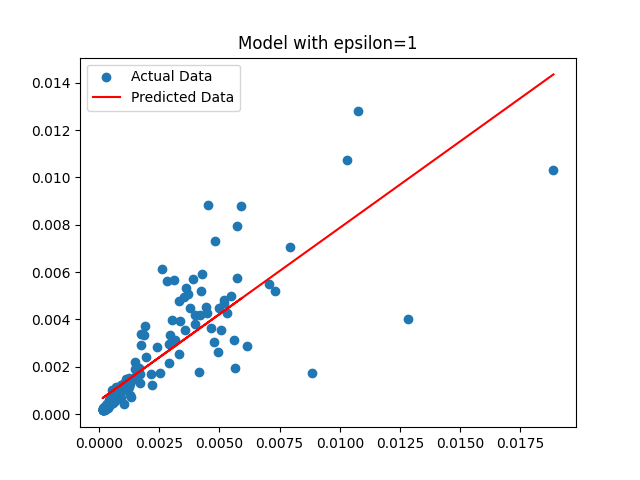
\includegraphics[width=.8\linewidth]{plots/epsilon_1}
            \caption{Caption for plot 1}
        \end{subfigure} \quad
        \begin{subfigure}[b]{0.3\textwidth}
            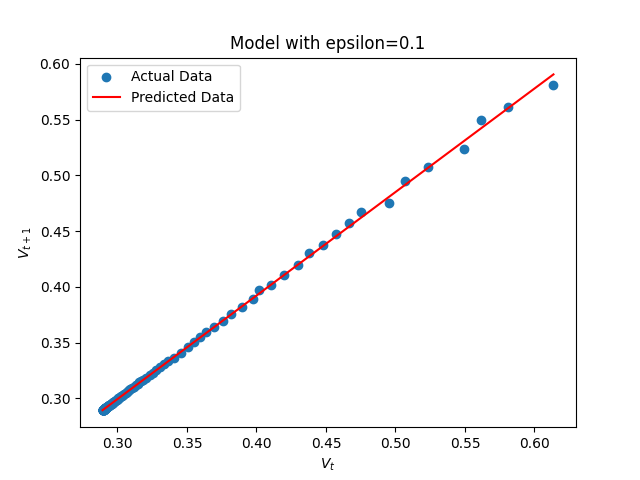
\includegraphics[width=.8\linewidth]{plots/epsilon_0.1}
            \caption{Caption for plot 2}
        \end{subfigure} \quad
        \begin{subfigure}[b]{0.3\textwidth}
            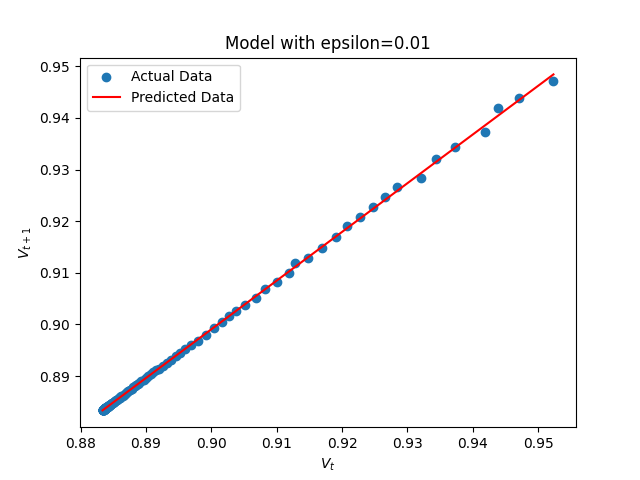
\includegraphics[width=.8\linewidth]{plots/epsilon_0.01}
            \caption{Caption for plot 3}
        \end{subfigure}\\
        \begin{subfigure}[b]{0.3\textwidth}
            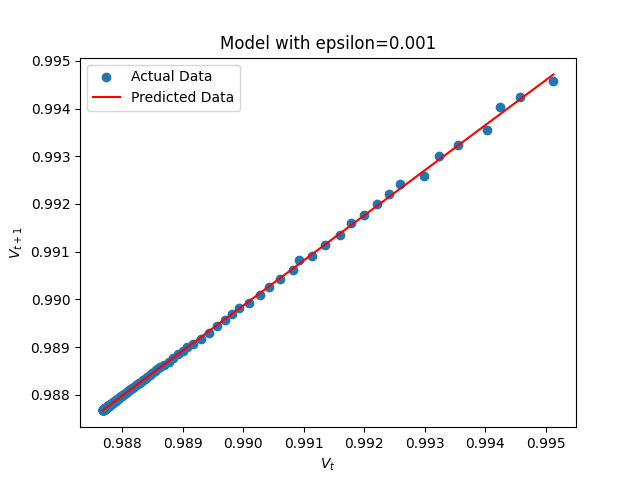
\includegraphics[width=.8\linewidth]{plots/epsilon_0.001}
            \caption{Caption for plot 4}
        \end{subfigure} \quad
        \begin{subfigure}[b]{0.3\textwidth}
            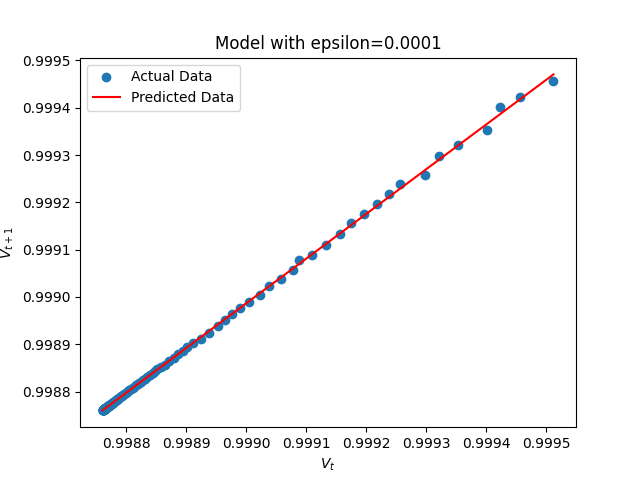
\includegraphics[width=.8\linewidth]{plots/epsilon_0.0001}
            \caption{Caption for plot 5}
        \end{subfigure}
        \caption{Regression Plot}
    \end{figure}

    \begin{table}[h!]
\label{tab:preliminary-regression}
\centering
    \begin{tabular}{llllll}
    \hline
                   & \varepsilon =: 1.0 & \varepsilon =: 0.1 & \varepsilon =: 0.01 & \varepsilon =: 0.001 & \varepsilon =: 0.0001  \\
    \hline
    $\beta_0$      & 0.0000*            & 0.0211***          & 0.0501***           & 0.0547***            & 0.0552***              \\
                   & (0.0000)           & (0.0006)           & (0.0013)            & (0.0014)             & (0.0014)               \\
    $\beta_1$      & 0.6348***          & 0.9278***          & 0.9433***           & 0.9446***            & 0.9447***              \\
                   & (0.0071)           & (0.0019)           & (0.0014)            & (0.0014)             & (0.0014)               \\
    \hline
    R-squared      & 0.9827             & 0.9994             & 0.9997              & 0.9997               & 0.9997                 \\
    R-squared Adj. & 0.9826             & 0.9994             & 0.9997              & 0.9997               & 0.9997                 \\
    N              & 142                & 142                & 142                 & 142                  & 142                    \\
    \hline
    \end{tabular}
    \caption{Standard errors in parentheses. \newline
$* p<0.1$, $** p<0.05$, $***p<0.01$}
\end{table}
\bigskip



    \subsection{GMM estimation with Stata}

    Let's consider the model:
    \begin{equation}
        N_{t} = \alpha_1 N_{t-1} + \alpha_2 N_{t-1}^{1 + \varepsilon} + U_t\label{eq:equation1}
    \end{equation}

    We assume that $U_t$ is mean independent of all the $N_s$ for $s\leq t-1$. For 3 parameters, at least 3 instruments are needed:

    \begin{table}[htbp]\centering
\def\sym#1{\ifmmode^{#1}\else\(^{#1}\)\fi}
\caption{GMM Regression Table}
\begin{tabular}{l*{4}{c}}
\hline\hline
                    &\multicolumn{1}{c}{(1)}&\multicolumn{1}{c}{(2)}&\multicolumn{1}{c}{(3)}&\multicolumn{1}{c}{(4)}\\
                    &\multicolumn{1}{c}{N\_1 N\_2}&\multicolumn{1}{c}{N\_1 N\_2 N\_3}&\multicolumn{1}{c}{N\_1 N\_2 N\_3 N\_4}&\multicolumn{1}{c}{N\_1 N\_2 N\_3 NlnN}\\
\hline
alpha1              &                     &                     &                     &                     \\
Constant            &       4.280         &       7.049         &       7.457         &       7.503         \\
                    &     (6.681)         &         (.)         &         (.)         &         (.)         \\
\hline
alpha2              &                     &                     &                     &                     \\
Constant            &      -2.528         &      -4.981\sym{***}&      -5.466\sym{***}&      -5.474\sym{***}\\
                    &     (6.514)         &    (0.0550)         &    (0.0453)         &    (0.0493)         \\
\hline
epsilon             &                     &                     &                     &                     \\
Constant            &      0.0210         &      0.0157\sym{***}&      0.0135\sym{***}&      0.0140\sym{***}\\
                    &    (0.0436)         &  (0.000896)         &  (0.000672)         &  (0.000730)         \\
\hline
J                   &  16240992.8         & 252496718.1         & 161236752.4         & 209017433.8         \\
J\_df                &           0         &           2         &           3         &           3         \\
rank                &           3         &           2         &           2         &           2         \\
\hline\hline
\multicolumn{5}{l}{\footnotesize Standard errors in parentheses}\\
\multicolumn{5}{l}{\footnotesize \sym{*} \(p<0.05\), \sym{**} \(p<0.01\), \sym{***} \(p<0.001\)}\\
\end{tabular}
\end{table}



    \subsection{Ramsay Test}




% \dot V(t) = -r\varepsilon\, \left(V_0-K^{-1}\right)e^{-r\varepsilon t}

For P-0 consider the stationary distribution as $t \to \infty $ and estimate t* as an average with that distribution